\documentclass[12pt]{article}
\usepackage[utf8]{inputenc}
\usepackage{float}
\usepackage{amsmath}
\hbadness=10000

\usepackage[hmargin=3cm,vmargin=6.0cm]{geometry}
%\topmargin=0cm
\topmargin=-2cm
\addtolength{\textheight}{6.5cm}
\addtolength{\textwidth}{2.0cm}
%\setlength{\leftmargin}{-5cm}
\setlength{\oddsidemargin}{0.0cm}
\setlength{\evensidemargin}{0.0cm}

%misc libraries goes here
\usepackage{tikz}
\usetikzlibrary{automata,positioning}

\begin{document}

\section*{Student Information } 
%Write your full name and id number between the colon and newline
%Put one empty space character after colon and before newline
Full Name :  Yasin Fatih ALPUL\\
Id Number :  2098739\\

% Write your answers below the section tags
\section*{Answer 1}
\subsection*{a.}
Let $G=(V,\Sigma, R, S)$ be any CFG, then $M=(K, \Sigma, \Gamma, \Delta, p, F)$ is a bottom-up parser PDA for M where $K=\{p,q\}$, $\Gamma=V$, $F=\{q\}$ and $\Delta$ contains the following.
\begin{itemize}
    \item $((p,a,e),(p,a))$ for each $a\in\Sigma$
    \item $((p,e,\alpha^R), (p, A))$ for each rule $A\rightarrow \alpha$ in R
    \item $((p,e,S), (q,e))$
\end{itemize}
Using this method, we define $M=(\{p,q\},\{a,b,c\}, \{S,X,a,b,c\},\Delta, p, \{q\})$ be a bottom up parser for G where $\Delta$ includes,
\begin{enumerate}
    \item $((p,a,e), (p,a))$
    \item $((p,b,e), (p,b))$
    \item $((p,c,e), (p,c))$
    \item $((p,e,XaXSa), (p,S))$
    \item $((p,e,XbXSb), (p,S))$
    \item $((p,e, c), (p, S))$
    \item $((p,e, Xa), (p, X))$
    \item $((p,e,Xb), (p,X))$
    \item $((p,e,e), (p, X))$
    \item $((p,e,S), (q,e))$
\end{enumerate}

\subsection*{b.}
\begin{align*}
    (p, abbcbabbaa, e) &\vdash_M (p, bbcbabbaa, a)\\
    &\vdash_M (p,bcbabbaa, ba)\\
    &\vdash_M (p,cbabbaa, bba)\\
    &\vdash_M (p,babbaa,cba)\\
    &\vdash_M (p,babbaa,Sba)\text{ used rule 6}\\
    &\vdash_M (p,abbaa,bSba)\\
    &\vdash_M (p,bbaa,abSba)\\
    &\vdash_M (p,bbaa,XabSba)\text{ used rule 9}\\
    &\vdash_M (p,bbaa,XbSba)\text{ used rule 7}\\
    &\vdash_M (p,bbaa,XSba)\text{ used rule 8}\\
    &\vdash_M (p,baa, bXSba)\\
    &\vdash_M (p,aa,abXSba)\\
    &\vdash_M (p,aa,XabXSba)\text{ used rule 9}\\
    &\vdash_M (p,aa,XbXSba)\text{ used rule 7}\\
    &\vdash_M (p,aa,Sa)\text{ used rule 5}\\
    &\vdash_M (p,aa,XSa)\text{ used rule 9}\\
    &\vdash_M (p,a,aXSa)\\
    &\vdash_M (p,e,aaXSa)\\
    &\vdash_M (p,e,XaaXSa)\text{ used rule 9}\\
    &\vdash_M (p,e,XaXSa)\text{ used rule 7}\\
    &\vdash_M (p,e,S)\text{ used rule 4}\\
    &\vdash_M (q,e,e)
\end{align*}


\section*{Answer 2}

\subsection*{a.}
%Do not submit solutions for b, yet solve it to prepare for the final.
There are two different cases which are the input being odd or even. It can be determined which one is the case by simply having two states and alternating between these two states as we go right. Say we have states $o$ (odd) and $e$ (even), the first case is simple.
\begin{enumerate}
    \item The machine went all the way and the head is at the rightmost $1$
    \item At this time, the machine is in the $e$ state, it switches to $o$ state by going right and landing at $\sqcup$
    \item Now, it is known to the machine that the $x$ is odd, so it writes a $1$ in place of $\sqcup$ then it halts
\end{enumerate}
The second case is slightly different, needing additional states. The machine repeatedly executes the following steps.
\begin{enumerate}
    \item The machine is at the immediate right of the right-most $1$, in state $e$
    \item The machine moves left and deletes the $1$ there, by writing $\sqcup$ instead
    \item Then it goes full left until it finds the $\sqcup$ symbol or the $x$ symbol
    \item Then it goes one square right and marks there, by writing $x$ instead, if it is a $1$
    \item Otherwise, at that moment, the machine deleted the second half of the $1$ symbols and has written $x$'s for the first half of the $1$ symbols
    \item This time, machine switches to a new state and re-writes $1$'s instead of $x$'s as it goes left until it hits the $\sqcup$ symbol after which it halts
\end{enumerate}
Below is a formal description for the machine that have been mentioned.\\
Let $M=(K,\Sigma,\Delta, s, H)$ be a Turing Machine where,
\begin{align*}
    K &= \{i,e,o,d,l,w,r,c,h\}\\
    &~~~~~\textit{(i for initial, d for delete, l for left,}\\
    &~~~~~\textit{w for write, r for right, c for change)}\\
    \Sigma &= \{1,x,\sqcup,\triangleright\}\\
    s &= i\\
    H &= \{h\}
\end{align*}
$\delta$ is given in the following table.
\begin{table}[H]
    \centering
    \begin{tabular}{c|c|c}
         $q$    &$\sigma$   &$\delta(q,\sigma)$\\\hline
         $i$    &$\sqcup$   & $(i,\sqcup, \rightarrow)$\\
         $i$    &$1$        &$(o,1,\rightarrow)$\\
         $o$    &$1$        &$(e,1,\rightarrow)$\\
         $e$    &$1$        &$(o,1,\rightarrow)$\\
         $o$    &$\sqcup$   &$(h,1,\rightarrow)$\\
         $e$    &$\sqcup$   &$(d,\sqcup,\leftarrow)$\\
         $d$    &$1$        &$(l,\sqcup,\leftarrow)$\\
         $l$    &$1$        &$(l,1,\leftarrow)$\\
         $l$    &$x$        &$(w,x,\rightarrow)$\\
         $l$    &$\sqcup$   &$(w,\sqcup,\rightarrow)$\\
         $w$    &$1$        &$(r,x,\rightarrow)$\\
         $r$    &$1$        &$(r,1,\rightarrow)$\\
         $r$    &$\sqcup$   &$(d,\sqcup,\leftarrow)$\\
         $d$    &$x$        &$(c, 1, \leftarrow)$\\
         $c$    &$x$        &$(c, 1, \leftarrow)$\\
         $c$    &$\sqcup$   &$(h, \sqcup,\rightarrow)$
    \end{tabular}
\end{table}
\section*{Answer 3}
Such a machine would only go right linearly. Even if it writes something to the input tape, it cannot go back and remember it. Thus, such a machine would have no means of memory and the set of languages it decides would be only regular languages.\\
To see this, we can say that such a machine has two operations. It can either stay put or go right. Even if it writes to the tape, it is not possible to recall what has been written. The stay put operation can be simulated by the e-moves of NFA. Moreover, the go right operation can be simulated by NFA reading its input. Since we know that NFA can decide if a language is regular, such a machine decides the set of regular languages.

\section*{Answer 4}

\subsection*{a.}
We can define a Queue-based TM by 5-tuple $M=(K,\Sigma, \Delta, s, H)$,  where $K$ is the set of finite control states, $\Sigma$ is the input alphabet. Note that $\Sigma \cap \{\#,\$,\sqcup\}=\emptyset$ because they are necessary for the computation of the machine. $s$ is the starting state such that $s\in K$, and $H$ is the halting states such that $H\subseteq K$. The machine halts when it landed on this state. Moreover, $\Delta$ denotes the transition function, from $(K-H)\times \Sigma\cup\{e\} \times \Sigma\cup\{e\}$ to $K \times \Sigma\cup\{e\}$. One thing to point out is the domain of the function includes $K-H$ instead of $K$ since it no longer makes any computation once it reaches some halting state. Moreover, function domain includes two $\Sigma$s because we need the conditions of both heads. We allow it to be $e$ so we do not need to dequeue something each time we make a computation. The function range includes one $\Sigma$ denoting the input to enqueue. Once again, we allow $e$ to not be forced to enqueue at every step.
\subsection*{b.}
The configuration is a 2-tuple such that $C\subseteq (K\times\Sigma^*)$. Here, $K$ denotes the state in which the machine currently at.  For instance, let $C_1 = (q, awb)$ where $q\in K$, $a,b\in\Sigma$ and $w\in\Sigma^*$. $a$ and $b$ denotes the front and rear of the input tape, respectively.
\subsection*{c.}
We define $\vdash_M$ to be the yields-in-one-step relation of the machine M. It is defined as $K\times \Sigma^*$ to $K\times\Sigma^*$ such that  $K$ denotes the state of the machine and $\Sigma^*$ denotes the input tape. For instance $(q, abwc)\vdash_M(p, bwc)$ is the dequeue operation where the front of tape is changed from $a$ to $b$. Moreover, $(q,awb)\vdash_M (p, awbc)$ is the enqueue operation where the rear of the machine is changed from $b$ to $c$. The reflexive, transitive closure of the relation, $\vdash^*_M$, yields the configuration of the machine after many steps. Let $L=L(M)$ be the language accepted by the machine. Then $w\in L$ if and only if machine makes a computation such as $(s,w)\vdash^*_M(q,w')$ where $s$ is the starting state, $q\in H$ and the heads of the machine initially points to the front and rear of the input tape.
\subsection*{d.}
We can show that a Turing Machine can simulate a Queue-based Turing Machine. But this makes it at least as powerful as the Queue-based TM. In order to show the equivalence, we need to show that a Queue-based TM can simulate a TM too.
A Turing Machine can simulate a Queue-based TM as the following,\\
A TM has three basic operations on an input tape. These are 'go left', 'go right' and 'write to tape'. Using these building blocks, we can simulate a Queue-based TM. Let $w$ be some arbitrary input where $w\in \Sigma^*$. Note that $\#,\$, \sqcup\notin \Sigma$. Before feeding it to a TM, we put $\#$ and $\$$ to both ends of the input. Thus, a TM can easily simulate the front and rear operations i.e by simply searching for $\#$ symbol and going right of it and conversely searching for $\$$ and going left of it. Enqueue operation is done by searching for $\$$ symbol, writing the symbol to be enqueued to there, going right and writing $\$$. On the other hand, dequeue operation is done by searching for the $\#$ symbol, writing $\sqcup$ there, going right and writing $\#$.\\
A queue-based can simulate a Turing machine as the following,\\
Since a TM has three operations, namely, 'go left', 'go right' and 'write to tape', we need to simulate these operations by a queue-based TM. Let the front of a queue-based TM always point to the head  of TM. We can easily simulate the 'go right' operation by dequeueing the front symbol and enqueueing it back at the rear. Conversely, to simulate a 'go left' operation, we need a slightly modified version of normal operations. Normally, the left of the head is on the left of the $\$$ symbol, the rear. Thus, we need to keep dequeueing and enqueueing. But we do not want to lose the marker. So without loss of generality, we can use a different symbol $\sigma\notin \Sigma$ only for this operation. Hence $\$$ symbol also gets carried all the way to the head. When we see it, we know what the rear symbol was. Note that we have a finite control states. Since $\Sigma$ is finite, we can have a state for each of the symbols as a \textit{buffer} to remember the symbol. Then we write the symbol in place of $\$$ and fix the other back head symbol accordingly to keep the machine stable. 'write to tape' operation is also trivial. We could simply ignore the symbol at the front head and enqueue the symbol to be written. Then, make it the new head using a series of enqueueing and dequeueing.\\
Hence, queue-based TM is equiavalent to Turing Machine.
\subsection*{e.}
Let $M=(K,\Sigma, \Delta, s, H)$ where
\begin{align*}
    K &= \{q_0, q_a, q_b, q_{ac}, q_{bc}, y,n\}\\
    \Sigma &= \{a,b\}\\
    s &= q_0\\
    H &= \{y, n\}
\end{align*}
$\Delta$ is given by the following table:\\
\begin{table}[H]
    \centering
    \begin{tabular}{c|c|c|c}
     q&f&b&$\Delta(q,f,b)$  \\\hline
     $q_0$&a&e&$(q_a, e)$ \\
     $q_0$&b&e&$(q_b,e)$ \\
     $q_0$&c&c&$(y,e)$\\
     $q_a$&a&e&$(q_a,a)$\\
     $q_a$&b&e&$(q_a,b)$\\
     $q_b$&a&e&$(q_b,a)$\\
     $q_b$&b&e&$(q_b,b)$\\
     $q_a$&c&e&$(q_{ac}, c)$\\
     $q_b$&c&e&$(q_{bc}, c)$\\
     $q_{ac}$&a&e&$(q_0,e)$\\
     $q_{bc}$&b&e&$(q_0,e)$\\
     $q_{ac}$&b&e&$(n,e)$\\
     $q_{bc}$&a&e&$(n,e)$
\end{tabular}
\end{table}

The idea is to start at the initial state $q_0$, eat up all the input in a cyclic manner till only the $c$ symbol remains. Let us assume the first symbol has been read is $a$, the other case is similar.\\
\begin{itemize}
    \item buffer it in the state $q_a$ then dequeue the symbol
    \item look for a $c$ while repeatedly enqueue and dequeue the symbols
    \item in the case of not finding a $c$, i.e landing at some $\sqcup$, go to state $n$ then halt
    \item when found $c$, go to state $q_{ac}$
    \item if the first symbol is an $a$, then dequeue it and go back to $q_0$ to start all over again
    \item if the symbol after the $c$ is not an $a$ go to $n$ then halt
    \item when both front and rear points at $c$ this means there is no symbol left so we halt at $y$
\end{itemize}
\section*{Answer 5}

\subsection*{a.}
The idea to be used in this machine is the following,
\begin{enumerate}
    \item Start at the beginning of the tape
    \item Read an $a$ symbol, write an $d$ in its place
    \item Go to the beginning of the sequence of $b$'s
    \item Mark every other $b$ symbol with $d$ symbols
    \item When reached to the sequence of $c$'s mark three consecutive $c$'s
    \item Go back to beginning and do it again
\end{enumerate}
By following this procedure, we decrease the number of $a$'s by one in each step while decreasing the number of $c$'s by three and halving the number of $b$'s. If at the end, no symbol left to read then we accept the language word, otherwise we reject. Below is a depiction of the machine.
\begin{center}
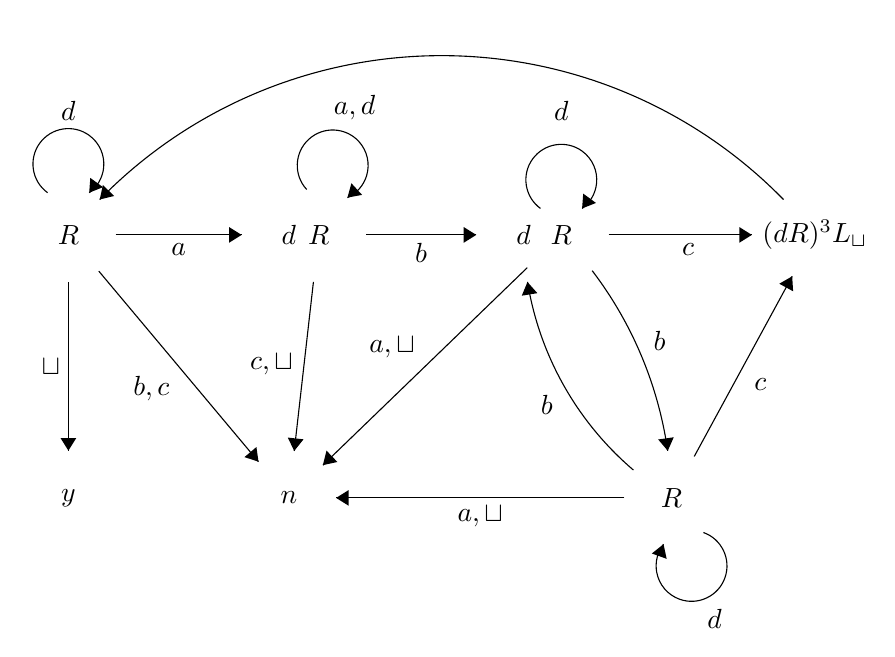
\begin{tikzpicture}[scale=0.2]
\tikzstyle{every node}+=[inner sep=0pt]
\draw (8.6,-16.5) node {$R$};
\draw (22.6,-16.5) node {$d$};
\draw (24.5,-16.5) node {$R$};
\draw (8.6,-33.2) node {$y$};
\draw (22.6,-33.2) node {$n$};
\draw (37.5,-16.5) node {$d$};
\draw (39.9,-16.5) node {$R$};
\draw (46.9,-33.2) node {$R$};
\draw (56,-16.5) node {$(dR)^3L_\sqcup$};
\draw [black] (11.6,-16.5) -- (19.6,-16.5);
\fill [black] (19.6,-16.5) -- (18.8,-16) -- (18.8,-17);
\draw (15.6,-17) node [below] {$a$};
\draw [black] (7.277,-13.82) arc (234:-54:2.25);
\draw (8.6,-9.25) node [above] {$d$};
\fill [black] (9.92,-13.82) -- (10.8,-13.47) -- (9.99,-12.88);
\draw [black] (8.6,-19.5) -- (8.6,-30.2);
\fill [black] (8.6,-30.2) -- (9.1,-29.4) -- (8.1,-29.4);
\draw (8.1,-24.85) node [left] {$\sqcup$};
\draw [black] (10.53,-18.8) -- (20.67,-30.9);
\fill [black] (20.67,-30.9) -- (20.54,-29.97) -- (19.78,-30.61);
\draw (15.05,-26.29) node [left] {$b,c$};
\draw [black] (23.729,-13.613) arc (222.69007:-65.30993:2.25);
\draw (26.77,-9.23) node [above] {$a,d$};
\fill [black] (26.32,-14.13) -- (27.25,-13.96) -- (26.57,-13.22);
\draw [black] (24.16,-19.48) -- (22.94,-30.22);
\fill [black] (22.94,-30.22) -- (23.53,-29.48) -- (22.53,-29.37);
\draw (22.89,-24.74) node [left] {$c,\sqcup$};
\draw [black] (27.5,-16.5) -- (34.5,-16.5);
\fill [black] (34.5,-16.5) -- (33.7,-16) -- (33.7,-17);
\draw (31,-17) node [below] {$b$};
\draw [black] (38.577,-14.82) arc (234:-54:2.25);
\draw (39.9,-9.25) node [above] {$d$};
\fill [black] (41.22,-14.82) -- (42.1,-14.47) -- (41.29,-13.88);
\draw [black] (41.859,-18.77) arc (37.31526:8.16787:24.653);
\fill [black] (46.66,-30.21) -- (47.04,-29.35) -- (46.05,-29.49);
\draw (45.73,-23.25) node [right] {$b$};
\draw [black] (48.925,-35.398) arc (70.38954:-217.61046:2.25);
\draw (49.63,-40.23) node [below] {$d$};
\fill [black] (46.39,-36.14) -- (45.65,-36.73) -- (46.59,-37.07);
\draw [black] (10.588,-14.255) arc (135.65096:44.34904:30.363);
\fill [black] (10.59,-14.25) -- (11.5,-14.03) -- (10.79,-13.33);
\draw [black] (37.74,-18.58) -- (24.76,-31.12);
\fill [black] (24.76,-31.12) -- (25.68,-30.92) -- (24.99,-30.2);
\draw (29.15,-24.37) node [above] {$a,\sqcup$};
\draw [black] (42.9,-16.5) -- (52,-16.5);
\fill [black] (52,-16.5) -- (51.2,-16) -- (51.2,-17);
\draw (47.95,-17) node [below] {$c$};
\draw [black] (48.34,-30.57) -- (54.56,-19.13);
\fill [black] (54.56,-19.13) -- (53.74,-19.6) -- (54.62,-20.08);
\draw (52.12,-26.03) node [right] {$c$};
\draw [black] (44.479,-31.433) arc (-130.4421:-170.80982:19.867);
\fill [black] (37.75,-19.49) -- (37.39,-20.36) -- (38.38,-20.2);
\draw (39.39,-27.27) node [left] {$b$};
\draw [black] (43.9,-33.2) -- (25.6,-33.2);
\fill [black] (25.6,-33.2) -- (26.4,-33.7) -- (26.4,-32.7);
\draw (34.75,-33.7) node [below] {$a,\sqcup$};
\end{tikzpicture}
\end{center}
\subsection*{b.}
Here is the idea for the unrestricted grammar to generate L
\begin{enumerate}
    \item Start with two anchor symbols on both ends, say $\#$(begin) and $\$$(end)
    \item Use a pivot going back and forth between two anchors
    \item The pivot should include the direction information in it, say $R$ for right and $L$ for left
    \item Use nonterminal symbols $A,B,C$ to generate the strings
    \item Generate one $A$  at the left end
    \item Double every $B$ in one pass
    \item Generate three $C$'s at the right end
    \item Change the direction to left and go left end to start again
    \item At the right end, nondeterministically, start converting $A,B,C$ to $a,b,c$ respectively
\end{enumerate}
\begin{align*}
    S &\rightarrow \#R\$\\
    \#R\$ &\rightarrow \#RABBCCC\$\\
    \#RA &\rightarrow \#AAR\\
    ARA &\rightarrow AAR\\
    ARB &\rightarrow ABBR\\
    BRB &\rightarrow BBBR\\
    BRC &\rightarrow BCR\\
    CRC &\rightarrow CCR\\
    CR\$ &\rightarrow CCCCL\$\\
    CL &\rightarrow LC\\
    BL &\rightarrow LB\\
    AL &\rightarrow LA\\
    \#L &\rightarrow \#R\\
    L\$ &\rightarrow T\\
    CT &\rightarrow Tc\\
    BT &\rightarrow Tb\\
    AT &\rightarrow Ta\\
    \#T &\rightarrow e\\
    S  &\rightarrow b\\
    S &\rightarrow abbccc
\end{align*}

\section*{Answer 6}

\subsection*{a.}
\-\hspace{1cm} $L_1$ is a regular language and is recognized by a finite automaton. Since Turing Machines are more powerful that finite automata, there is a Turing Machine accepting the same language $L_1$.\\
\-\hspace{1cm}
Similarly, $L_2$ and $L_3$ are context-free languages and are recognized by Pushdown automata. Since Turing machines are more powerful than Pushdown automata, there are Turing machines for each of the languages $L_2$ and $L_3$ that accepts them.\\
\-\hspace{1cm}The right side of the instersection is a complenet of a regular language, $a^*b^*$. Since we know that regular languages are closed under complement, by switching the accepting and non-accepting states, right side of the intersection is also regular. Hence, it can be simulated by a TM. Moreover, we can decide the intersection of two recursive languages. So, $\overline{L_4}$ must be recursive. To see this, observe that the intersection is said to be recursive. If the left side is not recursive, then the interseciton would not be recursive since both of them must be recursive. Since, complement of recursive languages are recursive, $L_4$ is recursive. We also know that recursive languages are decided by Turing machines. Hence, there is a TM that accepts $L_4$.\\
\-\hspace{1cm}Unrestricted grammars correspond to Turing machines. That is, there is a Turing machine for every unrestricted grammar that generates the same language, by nondeterministically trying the rules from the starting symbol and finishing with a tape that are all terminal symbols. Conversely, an unrestricted grammar can simulate the computation of a Turing machine by backwards execution. That is, Starting from the input tape at the halting state, $\triangleright\sqcup h\triangleleft$, reversing the operations of writing, going left and right and eventually finishing with $\triangleright\sqcup w\triangleleft\xrightarrow{G} w$. Hence, there is a Turing machine that accepts $L_5$.
\subsection*{b.}
\-\hspace{1cm}It is trivial for a Turing machine to simulate a finite automaton, it can just switch between states by not writing anything to the input tape. Hence, there is an algorithm for membership test for $L_1$.\\
\-\hspace{1cm}Similarly, Turing machine can also simply simulate PDA. It can be a 2-tape Turing machine, which there is an equivalent 1-tape standard machine, by simulating a stack in its second tape. Since, there is a deterministic parser for $L_2$, a TM can deterministically simulate it and make advancements in each step, reading input and applying rules on the stack. So, there is an algorithm for membership test for $L_2$. However, $L_3$ is inherently ambiguous and may not have a deterministic parser. So, it is not guaranteed to advance in every step, the machine may go in an infinite loop. If we come up with an algorithm, it would include guessing nondeterministically and may not halt at every computation.\\
\-\hspace{1cm} In part a, it is shown that $L_4$ is recursive. Hence, there is a TM that decides it. If the output of TM is y, then $w\in L_4$, else, $w\notin L_4$\\
\-\hspace{1cm} The decision problem of membership test that whether a word is in an unrestricted grammar is equivalent to whether it can be accepted by a TM equivalent to the grammar. That problem is called the Halting Problem and is undecidable. Recursively enumerable languages are generated by unrestricted grammars and they are only semidecided by TMs. A machine cannot know if it is ever going to halt on a computation. So, we may have to guess a transition at every step to show the membership but we may not always reach a halting state.
\subsection*{c.}
Let $T_1, T_2, T_3, T_4, T_5$ be the TM's for $L_1, L_2, L_3, L_4, L_5$, respectively. Properties of them and how to construct is explained in previous parts. In the case of $\overline{L_2}$, since the machine decides it, its complement can also be decided by a TM. For the $\overline{L_2}L_1$, the machine can split nondeterministically the given word and decide both parts. Let $w$ be the language we are trying to find whether $w\in L$ or not, the length of the word plus one $|w|+1$ is the number of possible splits. Since it is a finite number, the machince can guess the correct split nondeterministically and accept if some word $u\in\overline{L_2}L_1$ or not. Since TMs can simulate other TMs, let some machine M simulate both the machine for $\overline{L_2}L_1$ and $T_5$ in parallel, one alternating computation step for each.  If both of them halts at some point, then the machine accepts the word. Let this machine be called $Q$ such that $Q$ accepts some word $w$ if and only if $w\in\overline{L_2}L_1\cap L_5$ and say $N=\overline{L_2}L_1\cap L_5$. Another machine can accept the $N^*$ of this language by using $Q$. Since there is a finite number of splits for the given input word, say $w$, comprising of subwords $w_1w_2\dots w_n$, the machine nondeterministically guesses the correct split and accept each $w_i$ with $Q$. Let the resulting machine be $A$, we now continue with the second part, right side of $\cup$. Since $T_3$ accepts $L_3$, similar to the acceptance of $N^*$, some TM can guess the correct split and accept $L_3^*$. Moreover, because of $L_4$ being recursive, its complement is also recursive and can be decided by some TM. Let some other Turing Machine, say $B$, guesses the correct split between $L_3^*$ and $\overline{L_4}$ and accepts each individual part. Since $w\in L$ can be satisfied by accepting $w$ in either side of the union, some Turing Machine $X$ can simulate both $A$ and $B$ in parallel and hence $X$ accepts $L$. 
\subsection*{d.}
A TM semidecides a language $L$ if it is recursively enumerable. By previous parts, we showed that $L$ is recursively enumerable. Recursive languages are decided by TMs, i.e the machine halts on one of y or n state. It can be reverted, y becomes n and n becomes y, to decide the complement of the language. However, semideciding a language is accepted by halting at some state and rejected by running infinitely, and there is no way to revert that behaviour. Since recursively enumerable languages are not closed under complement, we cannot always come up with a TM to semidecide $\overline{L}$. 

%Do not submit solutions for Question 7, yet do solve it.


\end{document}